% !TeX root = ../thesis.tex

\chapter{Einleitung}
\label{sec:introduction}

Die Kommunikation über das Medium Licht ist eine neue und äußerst vielversprechende Technologie aus dem Bereich der optischen drahtlosen Kommunikation, die das sichtbare Spektrum für die Datenübertragung nutzt und sich aufgrund der hohen verfügbaren Bandbreite, des unregulierten sichtbaren Spektrums und der nicht vorhandenen elektromagnetischen Interferenzen als Lösung für Funkkommunikationssysteme herauskristallisierte. Daneben wird das \gls{acr:OFDM} als Modulationsverfahren für \gls{acr:VLC} verwendet, da es in der Lage ist, hohe Datenraten zu erzielen und gleichermaßen mit einer hohen spektralen Effizienz überträgt. Zudem werden mithilfe jener die Auswirkungen von Störungen durch \gls{acr:ISI} reduziert.

\section{Motivation}
\label{sec:motivation}

Der wachsende Drang in der heutigen Zeit mobil zu sein und ein Mobilfunkgerät zu besitzen führt dazu, dass Geräte die \gls{acr:HF}-bänder nutzen mit anderen Geräten interferieren. In modernen drahtlosen mobilen Telekommunikationssystemen sind die gängigsten Technologien der Zugangsnetze zur Datenübertragung die Funkfrequenzen. Mit der steigenden Nachfrage an Hochgeschwindigkeitsdatendiensten steigt die Auslastung \gls{acr:HF}-Spektrum. Darüber hinaus leidet die \gls{acr:HF}-basierte Kommunikation unter Mehrwegeausbreitung, was die Verfügbarkeit und Leistung von Verbindungen reduziert. Dies zusammen mit der Überlastung des \gls{acr:HF}-Spektrums bedeutet, dass nur wenige hochauflösende Kanäle in einem bestimmten Gebiet untergebracht werden können. Schätzungen zufolge belaufen sich etwa 70\% des drahtlosen Datenverkehrs in Innenräumen \cite{vlc2}, daher müssen Alternativen für drahtlose Kommunikationssysteme in speziell in Innenräumen in Betracht gezogen werden.
Eine solche Alternative sind \gls{acr:VLC}-Systeme, welche in ihren Anwendungsbereichen in Abbildung~\ref{fig:usecasevlc} illustriert werden. \gls{acr:VLC} nutzt das sichtbare Lichtspektrum  welches sich von 390- 700nm erstreckt und bietet daher im Vergleich zur \gls{acr:HF}-Kommunikation eine etwa zehntausend mal höhere Bandbreite in der Terahertz Größenordnung. 

\begin{figure}[H]
	\centering
	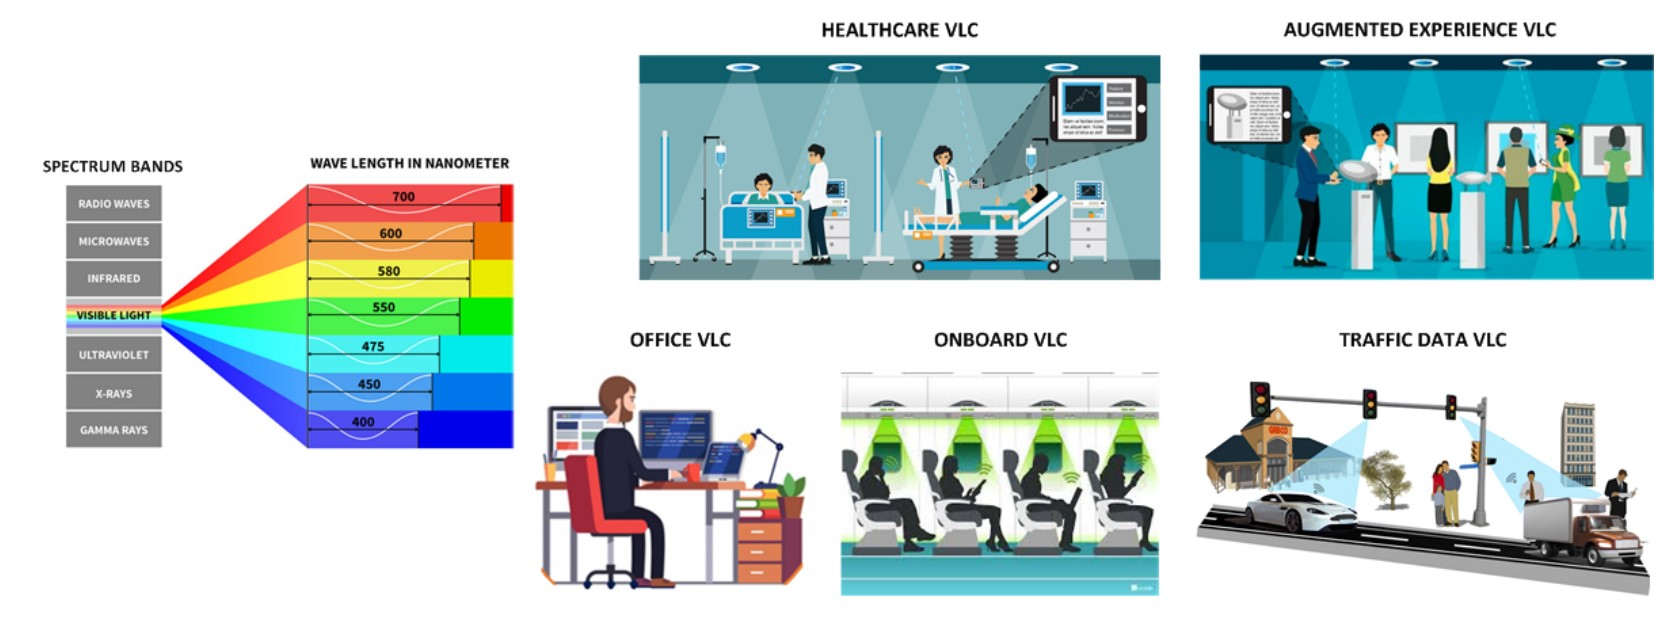
\includegraphics[width=1 \textwidth]{usecases.jpg}
	\caption[Wellenlänge und Use Cases von \gls{acr:VLC}]{Wellenlänge und Use Cases von \gls{acr:VLC}} 
	\cite{usecase}
	\label{fig:usecasevlc}
\end{figure}

Außerdem bietet es ein lizenzfreies Spektrum, nicht vorhandene elektromagnetische Interferenzen und eine erhöhte Sicherheit für Innenraumsysteme, da Licht auf die Dimensionen seines Ausleuchtungskegels beschränkt ist. Darüber hinaus gilt \gls{acr:VLC} als ökologische Technologie, da \gls{acr:LED}s energieeffiziente und leicht steuerbare Lichtquellen sind. Außerdem werden die Vorteile von bereits implementierten \gls{acr:LED} für einen doppelten Zweck der Beleuchtung und Datenkommunikation genutzt. Da moderne Kommunikationssysteme hohe Datenraten erfordern, muss ein Modulationsverfahren in Betracht gezogen werden, welches in der Lage ist, hohe Datenraten mit hoher spektraler Effizienz zu übertragen.\cite{VLC} Hierbei wurde \gls{acr:OFDM} gewählt, welches im Laufe dieser Abschlussarbeit noch weiter eingeleitet und ausgeführt wird.


\section{Ziel der Arbeit}
\label{sec:The aim of the work}


Ziel dieser Abschlussarbeit ist es, einen \gls{acr:VLC}-Sender mit einem variablen Offset für den Lichtstrom und einer automatischen Amplitudenregelung aufzubauen. Dieser soll es ermöglichen mittels modulierten Lichtwellen Audio Daten von \gls{acr:PC} zu \gls{acr:PC} zu übertragen. Dazu wurden folgende Rahmenbedingungen festgelegt: 

\begin{itemize}
	\item Simulation der analogen Signalverarbeitungsschaltung in LT-Spice
	\item Projektierung einer Platine für die Komprimierung der Schaltungsgröße
	\item Planung eines Gehäuses für die Unterbringung der Hardwarekomponenten
	\item Auseinandersetzung mit dem Thermischen Management
	\item Variabilität des Offsets
	\item Programmierung einer Automatischen Amplitudenregelung
	\item Modulation und Demodulation des Audio-Sendesignals mittels der Dream Software
\end{itemize}




\section{Vorgehensweise}
\label{sec:method}
Da es heutzutage immer mehr Funkgeräte im Privat- und Geschäftsbereich gibt,
kommt es vor, dass Geräte welche die selben Frequenzbänder nutzen sich gegenseitig
stören können. Beispiel dafür ist eine für den Fernseher ausgelegt Funkfernbedienung,
die bei der Bedienung zudem gleichzeitig die externe Musikanlage
ansteuert. Eine mögliche Lösung hierfür ist die Datenübertragung über ein anderes
Medium.

